\newpage
\section{Appendix}

\subsection{Dataset Details}
Our dataset is multi-faceted, comprising three distinct domains: Torch Hub, Tensor Hub, and HuggingFace. Each entry within this dataset is rich in detail, carrying critical pieces of information that further illuminate the nature of the data. Delving deeper into the specifics of each domain, Torch Hub provides 95 APIs. The second domain, Tensor Hub, is more expansive with a total of 696 APIs. Finally, the most extensive of them all, HuggingFace, comprises 925 APIs.

To enhance the value and utility of our dataset, we've undertaken an additional initiative. With each API, we have generated a set of 10 unique instructions. These instructions, carefully crafted and meticulously tailored, serve as a guide for both training and evaluation. This initiative ensures that every API is not just represented in our dataset, but is also comprehensively understood and effectively utilizable.

In essence, our dataset is more than just a collection of APIs across three domains. It is a comprehensive resource, carefully structured and enriched with added layers of guidance and evaluation parameters.

\paragraph{Domain Classification} The unique domain names encompassed within our dataset are illustrated in Figure~\ref{fig:domains}. The dataset consists of three sources with a diverse range of domains: Torch Hub houses 6 domains, Tensor Hub accommodates a much broader selection with 57 domains, while HuggingFace incorporates 37 domains. To exemplify the structure and nature of our dataset, we invite you to refer to the domain names represented in Figure~\ref{fig:data_exp}.

\paragraph{API Call Task} In this task, we test the model's capability to generate a single line of code, either in a zero-shot fashion or by leveraging an API reference. Primarily designed for evaluation purposes, this task effectively gauges the model's proficiency in identifying and utilizing the appropriate API call. 

\paragraph{API Provider Component} This facet relates to the provision of the programming language. In this context, the API provider plays a vital role as it serves as a foundation upon which APIs are built and executed.

\paragraph{Explanation Element} This component offers valuable insights into the rationale behind the usage of a particular API, detailing how it aligns with the prescribed requirements. Furthermore, when certain constraints are imposed, this segment also incorporates those limitations. Thus, the explanation element serves a dual purpose, offering a deep understanding of API selection, as well as the constraints that might influence such a selection. This balanced approach ensures a comprehensive understanding of the API usage within the given context.

\paragraph{Code} Example code for accomplishing the task. We de-prioritize this as we haven't tested the execution result of the code. We leave this for future works, but make this data available in-case others want to build on it.

\begin{figure}
\begin{tcolorbox}
    \textbf{Torch Hub domain names}: Classification, Semantic Segmentation, Object Detection, Audio Separation, Video Classification, Text-to-Speech
\end{tcolorbox}
\begin{tcolorbox}
    \textbf{Tensor Hub domain names}: text-sequence-alignment, text-embedding, text-language-model, text-preprocessing, text-classification, text-generation, text-question-answering, text-retrieval-question-answering, text-segmentation, text-to-mel, image-classification, image-feature-vector, image-object-detection, image-segmentation, image-generator, image-pose-detection, image-rnn-agent, image-augmentation, image-classifier, image-style-transfer, image-aesthetic-quality, image-depth-estimation, image-super-resolution, image-deblurring, image-extrapolation, image-text-recognition, image-dehazing, image-deraining, image-enhancemenmt, image-classification-logits, image-frame-interpolation, image-text-detection, image-denoising, image-others, video-classification, video-feature-extraction, video-generation, video-audio-text, video-text, audio-embedding, audio-event-classification, audio-command-detection, audio-paralinguists-classification, audio-speech-to-text, audio-speech-synthesis, audio-synthesis, audio-pitch-extraction
\end{tcolorbox}
\begin{tcolorbox}
    \textbf{HuggingFace domain names}: Multimodal Feature Extraction, Multimodal Text-to-Image, Multimodal Image-to-Text, Multimodal Text-to-Video, Multimodal Visual Question Answering, Multimodal Document Question Answer, Multimodal Graph Machine Learning, Computer Vision Depth Estimation, Computer Vision Image Classification, Computer Vision Object Detection, Computer Vision Image Segmentation, Computer Vision Image-to-Image, Computer Vision Unconditional Image Generation, Computer Vision Video Classification, Computer Vision Zero-Shor Image Classification, Natural Language Processing Text Classification, Natural Language Processing Token Classification, Natural Language Processing Table Question Answering, Natural Language Processing Question Answering, Natural Language Processing Zero-Shot Classification, Natural Language Processing Translation, Natural Language Processing Summarization, Natural Language Processing Conversational, Natural Language Processing Text Generation, Natural Language Processing Fill-Mask, Natural Language Processing Text2Text Generation, Natural Language Processing Sentence Similarity, Audio Text-to-Speech, Audio Automatic Speech Recognition, Audio Audio-to-Audio, Audio Audio Classification, Audio Voice Activity Detection, Tabular Tabular Classification, Tabular Tabular Regression, Reinforcement Learning Reinforcement Learning, Reinforcement Learning Robotics
\end{tcolorbox}
\caption{\textbf{Domain names}: Domain names with the three dataset. Tensor Hub is the smallest dataset while the other two hubs contain many more models.}
    \label{fig:domains}
\end{figure}


\begin{figure}
\begin{tcolorbox}
    \textbf{\#\#\# User}: Our customer is a zoo and we want to help them detect movement of different animals. Write a python program in 1 to 2 lines to call API in TensorFlowHub.
    
    \textbf{\#\#\# Assistant}: 
    
    \textbf{<domain>}: image-object-detection,
    
    \textbf{<api\_call>}: detector = hub.load('https://tfhub.dev/google/openimages\_v4/ssd\_mobilenet\_v2/1'),
    \textbf{<api\_provider>}: TensorFlow Hub,
    
    \textbf{<explanation>}: This API call loads the pre-trained Single Shot Detector (SSD) MobileNet V2 model from TensorFlow Hub, which has been trained on the Open Images v4 dataset. This model is used for object detection in images. Once loaded, you can pass an image (and an optional score threshold for detection confidence) to the detector to get back the detected objects along with their bounding boxes, class labels, and associated confidence scores.
    
    \textbf{<code>}: import tensorflow as tf; import tensorflow\_hub as hub; \# Load the SSD MobileNet V2 model; detector = hub.load('https://tfhub.dev/google/openimages\_v4/ssd\_mobilenet\_v2/1'); \# Use the model to detect objects in an image (assuming 'image' is a TensorFlow tensor representing your image); result = detector(image, score\_threshold=0.5)
\end{tcolorbox}
\begin{tcolorbox}
    \textbf{\#\#\# User}: I am an engineer at Uber and I need to find a API that can classify pedestrians, cars, etc. from an image of the scene. Write a python program in 1 to 2 lines to call API in TorchHub.

    \textbf{<Reference API>}: \{domain: Object Detection, framework: PyTorch, functionality: Traffic Object Detection, Drivable Area Segmentation, Lane Detection, api\_name: HybridNets, api\_call: torch.hub.load(repo\_or\_dir='datvuthanh/hybridnets', model='hybridnets', pretrained=True), api\_arguments: repo\_or\_dir, model, pretrained, python\_environment\_requirements: Python>=3.7, PyTorch>=1.10, example\_code: 'import torch; model = torch.hub.load('datvuthanh/hybridnets', 'hybridnets', pretrained=True); img = torch.randn(1,3,640,384); features, regression, classification, anchors, segmentation = model(img), performance: {dataset: [{name: BDD100K, accuracy: {Traffic Object Detection: {Recall (\%): 92.8, mAP@0.5 (\%): 77.3}, Drivable Area Segmentation: {Drivable mIoU (\%): 90.5}, Lane Line Detection: {Accuracy (\%): 85.4, Lane Line IoU (\%): 31.6}}}]}, description: HybridNets is an end2end perception network for multi-tasks. Our work focused on traffic object detection, drivable area segmentation and lane detection. HybridNets can run real-time on embedded systems, and obtains SOTA Object Detection, Lane Detection on BDD100K Dataset.\}

    \textbf{\#\#\# Assistant}: 
    
    \textbf{<domain>}: Object Detection, \textbf{<api\_call>}: model = torch.hub.load('datvuthanh/hybridnets', 'hybridnets', pretrained=True),
    
    \textbf{<api\_provider>}: PyTorch,
    
    \textbf{<explanation>}: Load the pretrained HybridNets model for object detection from PyTorch Hub to classify pedestrians, cars, etc. in an image of the scene, 
    
    \textbf{<code>}: import torch; model = torch.hub.load('datvuthanh/hybridnets', 'hybridnets', pretrained=True)
\end{tcolorbox}
    \caption{\textbf{Example of the Dataset}: Two examples of the dataset, the above one is zero-shot (without information retrievers) and the bottom one is with information retriever. }
    \label{fig:data_exp}
\end{figure}

\subsection{\gorilla{} Details}
We provide all the training details for \gorilla{} in this section. This includes how we divide up the training, evaluation dataset, training hyperparameters for \gorilla{}.

\paragraph{Data} For HuggingFace, we devise the entire dataset into 90\% training and 10\% evaluation. For Torch Hub and Tensor Hub, we devise the data in to 80\% training and 20\% testing. 

\paragraph{Training}
We train \gorilla for 5 epochs with the 2e-5 learning rate with cosine decay. The details are provide in Tab.~\ref{tab:hyperparameter}. We finetune it on 8xA100 with 40G memory each. 

\begin{table*}[!htb]
% \color{red}
\caption{Hyperparameters for training \gorilla{} }
\footnotesize
\setlength\tabcolsep{3.5pt}
\label{tab:hyperparameter}
\centering
\begin{tabular}{p{5cm}p{3cm}p{3cm}p{2.5cm}p{2.5cm}p{2cm}p{2cm}}
% {lcccccccccccc}
\toprule
Hyperparameter Name & Value \\ 
\midrule
learning rate & 2e-5 \\
batch size & 64 \\
epochs & 5 \\
warmup ratio & 0.03 \\
weight decay & 0 \\
max seq length & 2048 \\

\bottomrule 
\end{tabular}
\end{table*}



\subsection{Performance Comparison}
We provide a full comparison of each model's performance in this section. In Fig~\ref{fig:full1} and Fig.~\ref{fig:full2}, the full set of comparisons is provided. We see that especially in zero-shot case, \gorilla{} surpasses the GPT-4 and GPT-3.5 by a large margin. The GPT-4 and GPT-3.5 gets around 40\% accuracy in Torch Hub and Tensor Hub, which are two structured API calls. Compared to that, HuggingFace is a more flexible and diverse Hub, as a result, the performance on HuggingFace is not as competitive.

\subsubsection{Evaluation}
For ease of evaluation, we manually cleaned up the dataset to make sure each API call domain only contains the valid call in the form of: 
\begin{tcolorbox}
\centering
    API\_name(API\_$\mathrm{arg_{1}}$, API\_$\mathrm{arg_{2}}$, ..., API\_$\mathrm{arg_{k}}$)
\end{tcolorbox}
Our framework allows the user to define any combination of the arguments to check. For Torch Hub, we check for the API name \texttt{torch.hub.load} with arguments \texttt{repo\_or\_dir} and \texttt{model}. For Tensor Hub, we check API name \texttt{hub.KerasLayer} and \texttt{hub.load} with argument \texttt{handle}. For HuggingFace, since there are many API function names, we don't list all of them here. One specific note is that we require the \texttt{pretrained\_model\_name\_or\_path} argument for all the calls except for \texttt{pipeline}. For \texttt{pipeline}, we don't require the \texttt{pretrained\_model\_name\_or\_path} argument since it automatically select a model for you once \texttt{task} is specified.  

\subsubsection{Hallucination}
We found especially in HuggingFace, the GPT-4 model incurs serious hallucination problems. It would sometimes put a GitHub name that is not associated with the HuggingFace repository in to the domain of \texttt{pretrained\_model\_name\_or\_path}. Fig.~\ref{fig:hallucination} demonstrates some examples and we also observe that GPT-4 sometimes assumes the user have a local path to the model like \texttt{your\_model\_name}. This is greatly reduced by \gorilla{} as we see the hallucination error comparison in Tab.~\ref{tab:llm_eval}.

\begin{figure}
\begin{tcolorbox}
    generate\_video = pipeline("text-to-video", model="your\_model\_name")
\end{tcolorbox}
\begin{tcolorbox}
    vqa = pipeline("visual-question-answering", model="microsoft/clip-vqa-base", tokenizer="microsoft/clip-vqa-base")
\end{tcolorbox}
\begin{tcolorbox}
    depth\_estimator = pipeline("depth-estimation", model="intel-isl/MiDaS", tokenizer="intel-isl/MiDaS")
\end{tcolorbox}
    \caption{\textbf{Hallucination Examples}: GPT-4 incurs serious hallucination errors in HuggingFace. We show a couple of examples in the figure.}
    \label{fig:hallucination}
\end{figure}


\begin{figure}[t]
    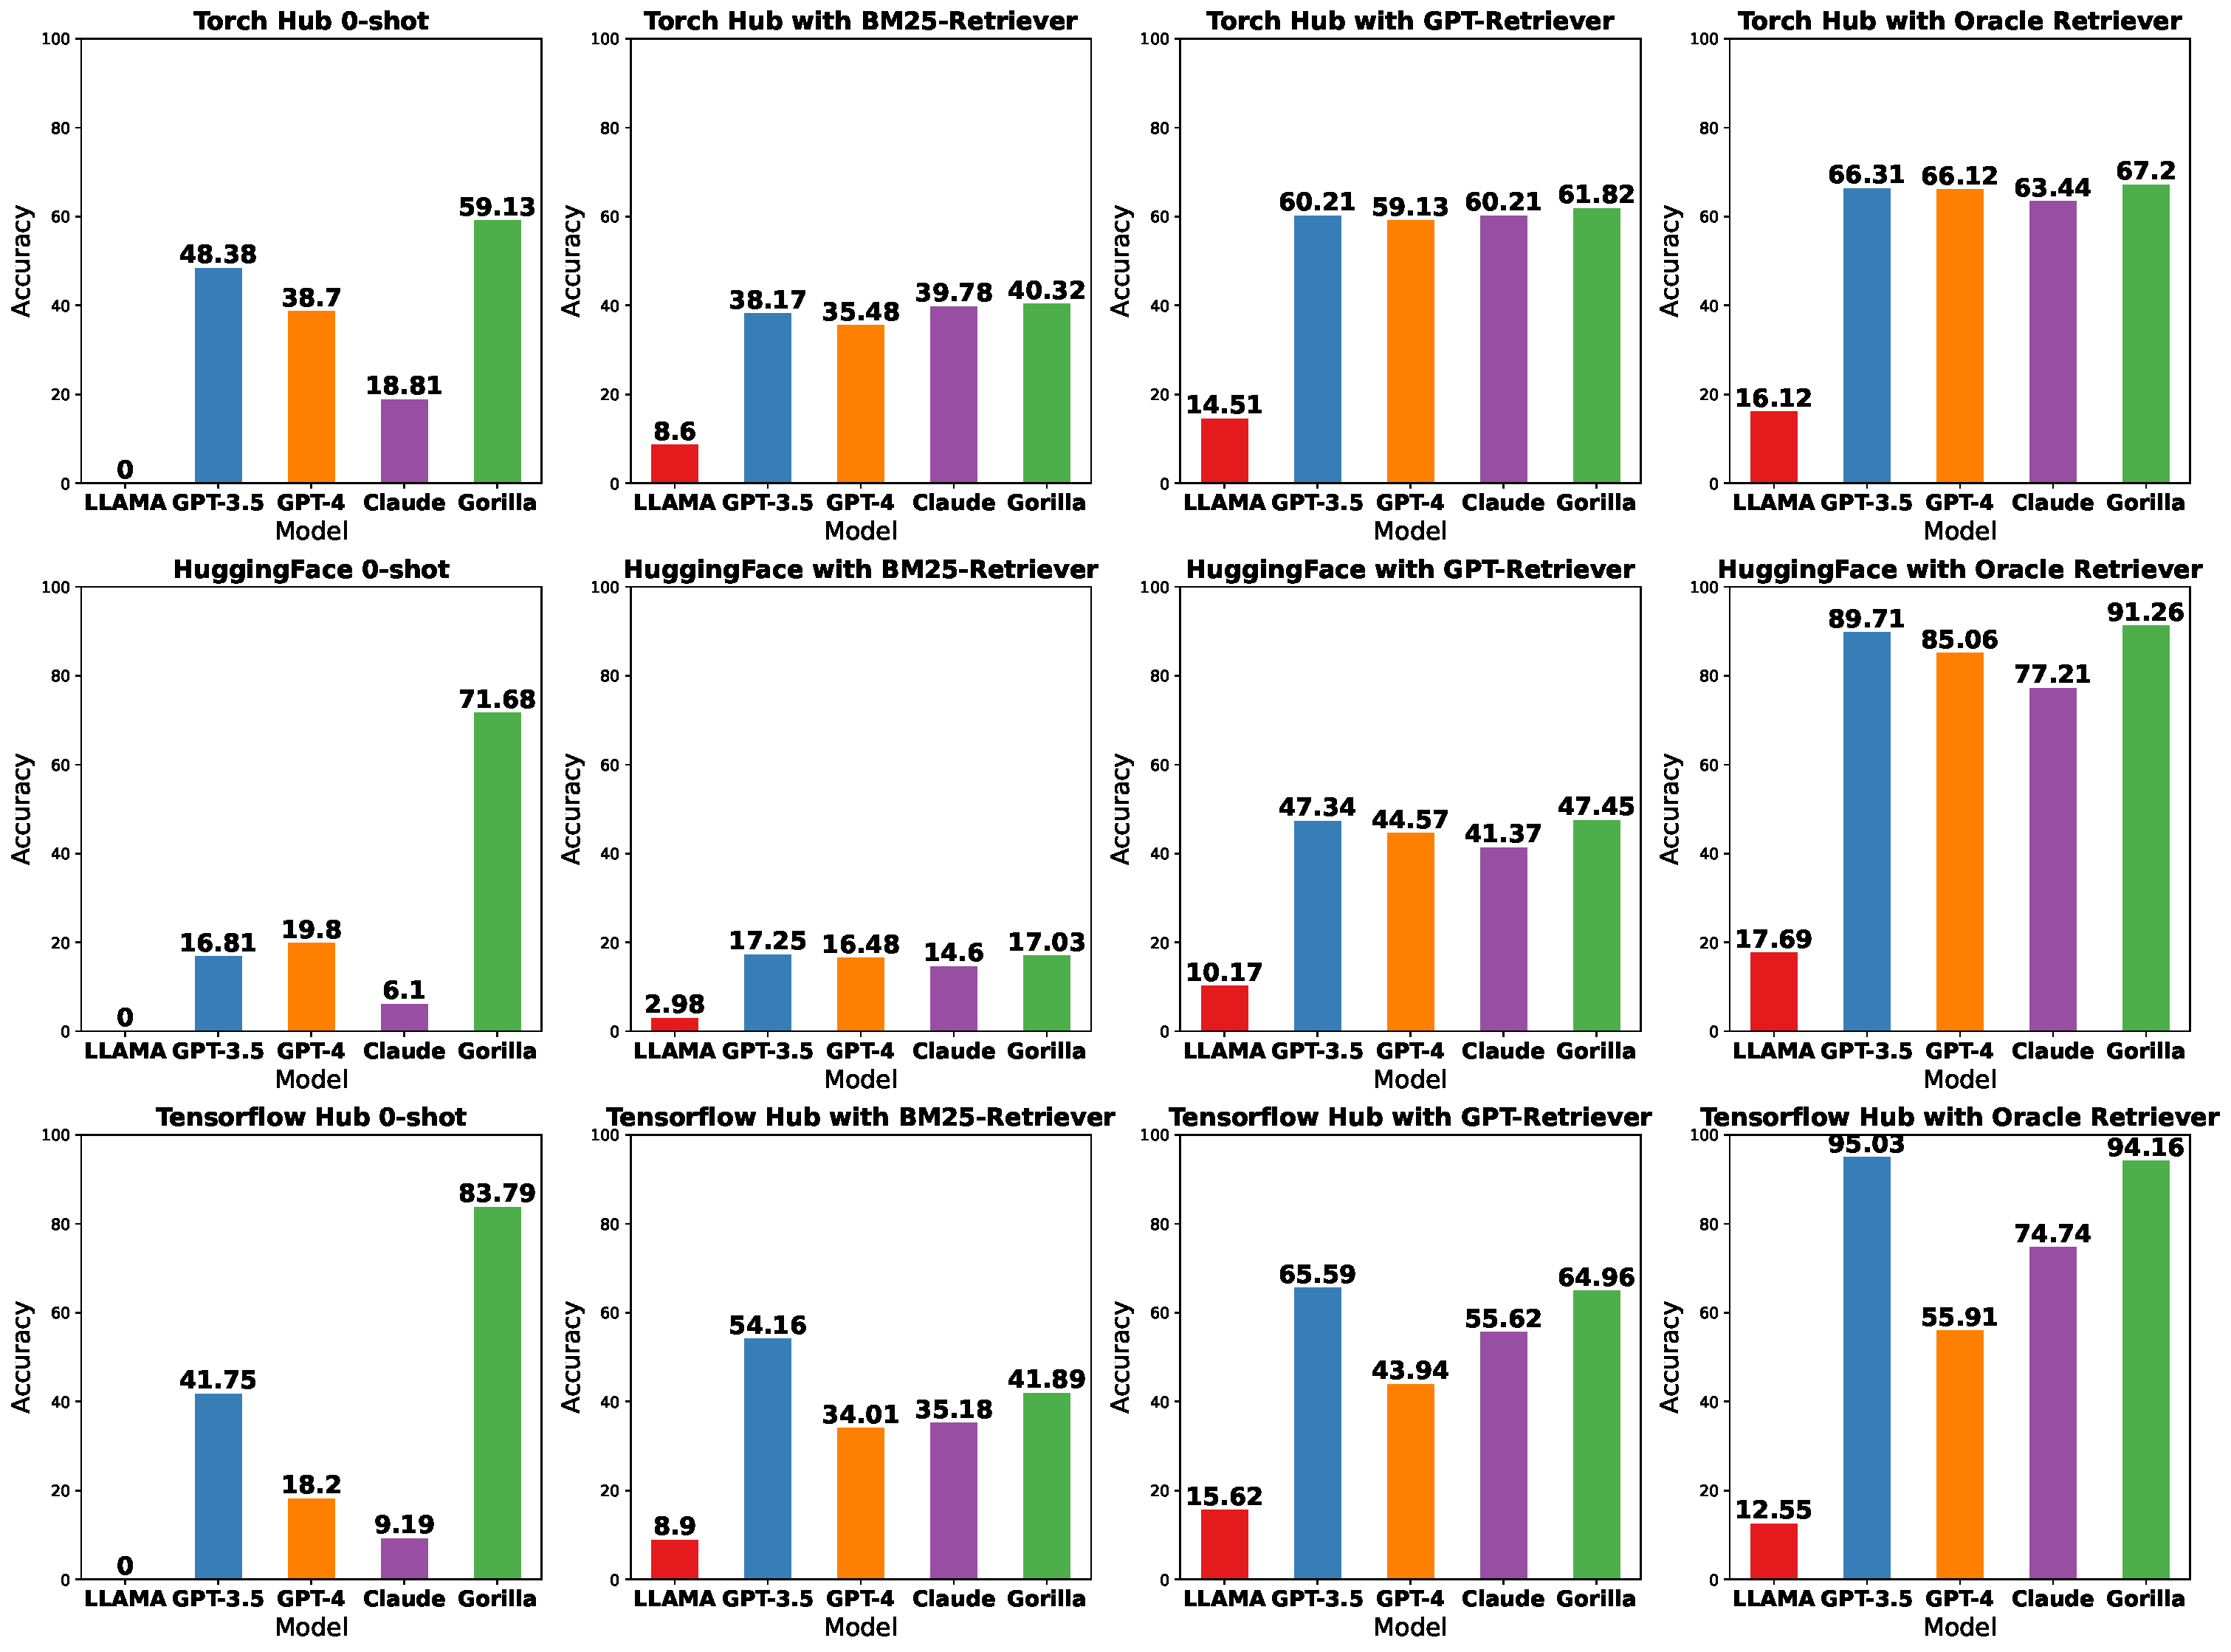
\includegraphics[width=\linewidth]{appendix_figures/grid_bars-3.pdf}
\caption{\footnotesize \textbf{ Performance}: We plot each model's performance on different configurations. We see that \gorilla{} performs extremely well in the zero-shot setting. While even when the oracle answer is given, \gorilla{} is still the best.}
\label{fig:full1}
\end{figure}

\begin{figure}[t]
    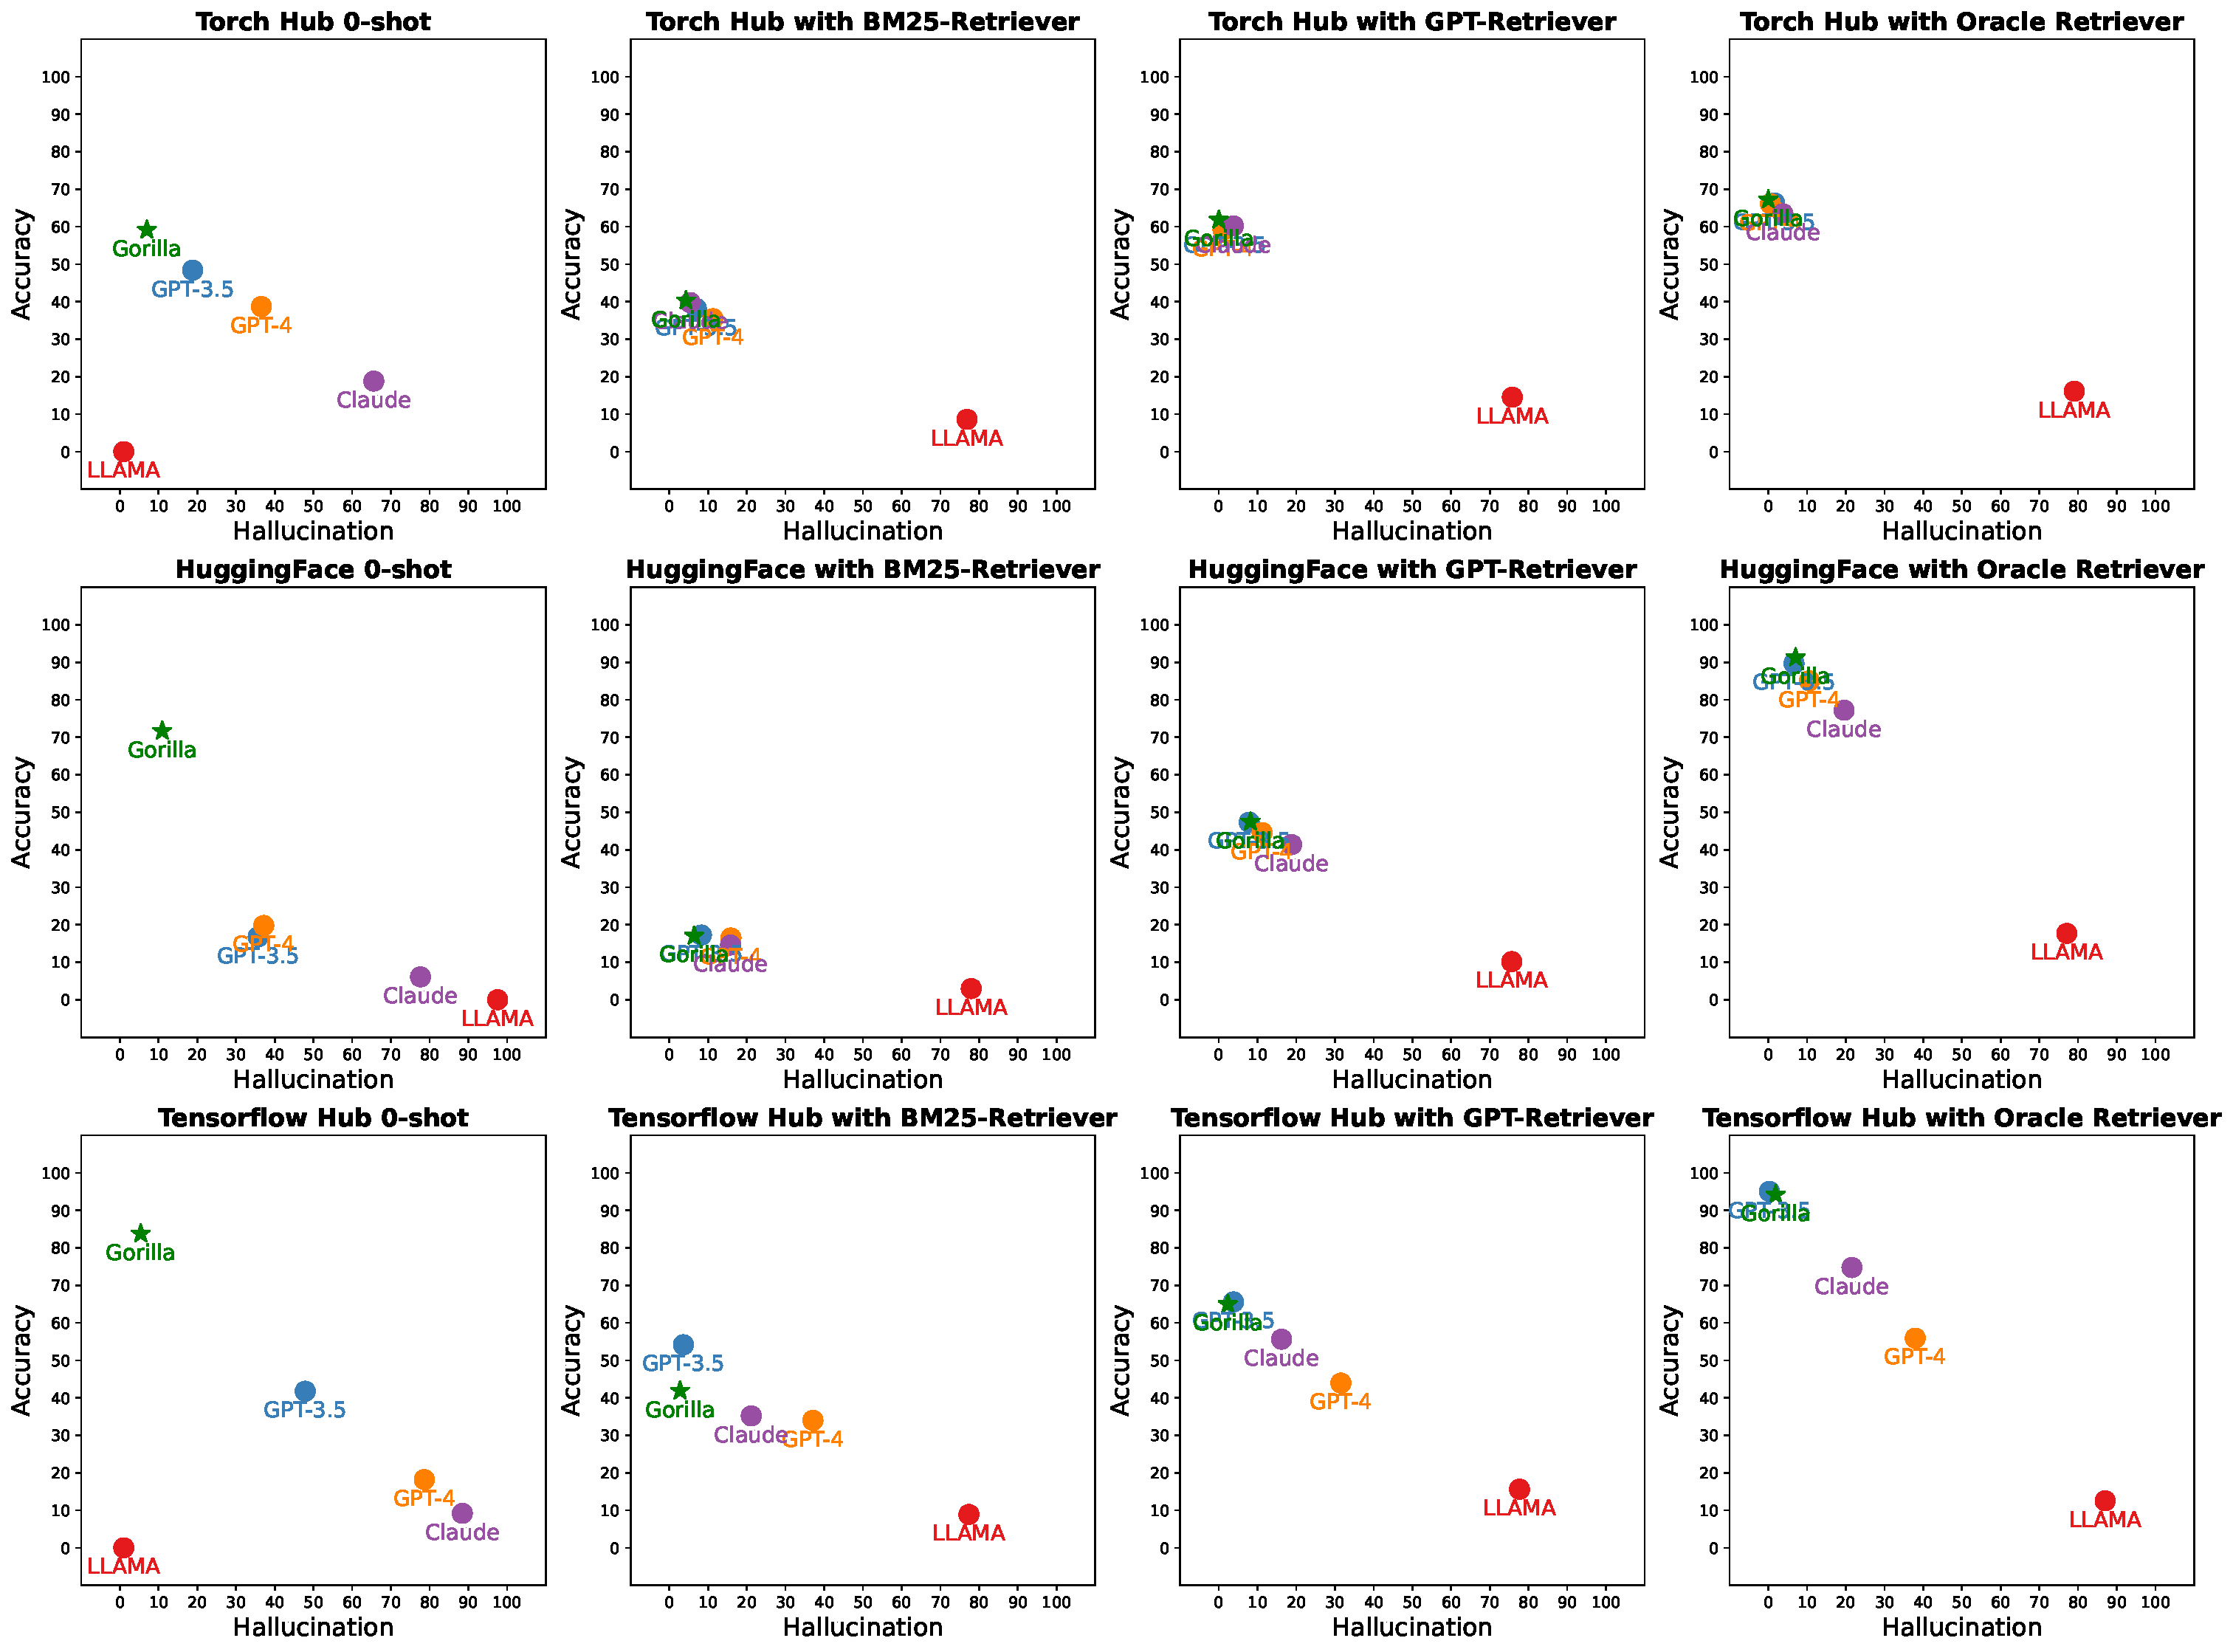
\includegraphics[width=\linewidth]{appendix_figures/grid-3.pdf}
\caption{\footnotesize \textbf{ Accuracy vs Hallucination}: We plot each model's performance on different configurations. We found that in the zero-shot setting, \gorilla{} has the most accuracy gain while maintaining good factual capability. When prompting with different retrievers, \gorilla{} is still capable to avoid the hallucination errors.}
\label{fig:full2}
\end{figure}